\documentclass[fontset=ubuntu]{ctexart}


% ------- 导入包 ------- %
\usepackage{hyperref}
\usepackage{fancyhdr}
\usepackage{tabularx}
\usepackage{graphicx}
\usepackage{amsmath}
\usepackage{multicol}
\usepackage{cite}

% ------- 页眉页脚设置 ------- %
\pagestyle{fancy}
\fancyhf{}
\fancyfoot[C]{\thepage}
\renewcommand{\headrulewidth}{0pt}
\renewcommand{\footrulewidth}{0pt}


% ------- 图片编号 ------- %

% ------- 标题页 ------- % 
\title{红酒质量分析报告}
\author{回归分析小组}
\date{\today}


% ------- 主文档 ------- %
\begin{document}

    % ------- 标题页 ------- %
    \maketitle
    \thispagestyle{empty}
    \newpage

    % ------- 目录页 ------- %
    \tableofcontents
    \thispagestyle{empty}
    \newpage
    \setcounter{page}{1} % 重置页码

    % ------- 正文 ------- %
    \section{问题背景}
        随着酒类产品在市场上的广泛受欢迎,对于酒的质量和特征的深入了解变得至关重要。为了更好地了解酒的品质,我们进行了一项回归分析,重点关注了酒的酸度,二氧化硫($SO_2$)含量等特征。这些特征在很大程度上影响了酒的口感、风味和保存能力。 

    \section{数据说明}
        我们通过 \href{https://archive.ics.uci.edu/dataset/186/wine+quality}{UC Irvine}仓库 ~\cite{cortez2009modeling} 下载了红酒数据,数据集中的特征包含酒的各类化学成分指标以及酒的品质评价。其中,成分指标,如$pH$值、$SO_2$含量、残糖量等通过物理化学检测得出;酒的品质由专业品酒师做出评价。(每个样本由三个品酒师做出评价,每个人的评分为$0$(差)到$10$(好)的一个整数,最终评价取三人的中位数)。红酒共$599$条数据,其中不含缺失值,共记录了$12$个特征,特征说明如 \ref{tab:features} 所示。

        \begin{table}[htbp]
            \centering
            \caption{酒的特征说明}
            \vspace{5pt}
            \begin{tabular}{cccc}
                \hline
                变量名 & 中文含义 & 变量类型 & 单位 \\
                \hline
                fixed acidity & 固定酸度 & 连续型变量 & g/L \\
                Volatile Acidity & 挥发性酸度 & 连续型变量 & g/L \\
                Citric Acid & 柠檬酸 & 连续型变量 & g/L\\
                Residual Sugar & 残糖 & 连续型变量 & g/L \\
                Chlorides & 氯化物 & 连续型变量 & g/L\\
                Free Sulfur Dioxide & 游离二氧化硫 & 连续型变量 & g/L \\
                Total Sulfur Dioxide & 总二氧化硫 & 连续型变量 & g/L \\
                Density & 密度 & 连续型变量 & g/mL \\
                pH &  葡萄酒的pH值 & 连续型变量 & \\
                Sulphates & 硫酸盐 & 连续型变量 & g/L \\
                Alcohol & 醇度 & 连续型变量 & \% \\
                Quality & 酒品 & 离散型变量 & \\ 
                \hline
            \end{tabular}
            \label{tab:features}
        \end{table}

    \section{描述性统计}
        \subsection{数值特征}
        对数据的初步描述如表 \ref{tab:description1-4},表\ref{tab:description5-8}和表\ref{tab:description9-12} 所示,包含平均值、最小值、最大值、中位数。
        \begin{table}[ht]
            \centering
            \caption{数据描述1-4}
            \vspace{5pt}
            \begin{tabular}{llll}
                \hline
                fixed.acidity & volatile.acidity &  citric.acid & residual.sugar \\ 
                \hline
                Min.   : 6.557   & Min.   :0.0052   & Min.   :-0.1331   & Min.   :1.223   \\ 
                1st Qu.: 7.857   & 1st Qu.:0.3278   & 1st Qu.: 0.3126   & 1st Qu.:1.784   \\ 
                Median : 8.622   & Median :0.4581   & Median : 0.4563   & Median :1.977   \\ 
                Mean   : 8.859   & Mean   :0.4808   & Mean   : 0.4535   & Mean   :2.407   \\ 
                3rd Qu.: 9.309   & 3rd Qu.:0.6300   & 3rd Qu.: 0.5803   & 3rd Qu.:2.457   \\ 
                Max.   :12.642   & Max.   :1.0396   & Max.   : 1.1742   & Max.   :6.780   \\ 
                \hline
            \end{tabular}
            \label{tab:description1-4}
        \end{table}

        \begin{table}[ht]
            \centering
            \caption{数据描述5-8}
            \vspace{5pt}
            \begin{tabular}{llll}
                \hline
                chlorides & free.sulfur.dioxide & total.sulfur.dioxide &    density \\ 
                \hline
                Min.   :-0.17986   & Min.   : 2.872   & Min.   :  9.874   & Min.   :0.7226   \\ 
                1st Qu.: 0.07193   & 1st Qu.: 8.041   & 1st Qu.: 24.112   & 1st Qu.:0.9328   \\ 
                Median : 0.16598   & Median :15.930   & Median : 56.041   & Median :0.9960   \\ 
                Mean   : 0.21012   & Mean   :16.475   & Mean   : 63.791   & Mean   :1.0014   \\ 
                3rd Qu.: 0.35014   & 3rd Qu.:22.089   & 3rd Qu.:102.992   & 3rd Qu.:1.0719   \\ 
                Max.   : 0.76331   & Max.   :39.160   & Max.   :151.197   & Max.   :1.2901   \\ 
                \hline
            \end{tabular}
            \label{tab:description5-8}
        \end{table}

        \begin{table}[ht]
            \centering
            \caption{数据描述9-12}
            \vspace{5pt}
            \begin{tabular}{llll}
                \hline
                pH &   sulphates &    alcohol &    quality \\ 
                \hline
                Min.   :2.611   & Min.   :-0.09304   & Min.   : 8.768   & Min.   :4.000   \\ 
                1st Qu.:3.017   & 1st Qu.: 0.34213   & 1st Qu.: 9.273   & 1st Qu.:5.000   \\ 
                Median :3.134   & Median : 0.50100   & Median : 9.498   & Median :5.000   \\ 
                Mean   :3.129   & Mean   : 0.64124   & Mean   : 9.888   & Mean   :5.581   \\ 
                3rd Qu.:3.256   & 3rd Qu.: 0.72854   & 3rd Qu.:10.346   & 3rd Qu.:6.000   \\ 
                Max.   :3.582   & Max.   : 2.84062   & Max.   :12.465   & Max.   :8.000   \\ 
                \hline
            \end{tabular}
            \label{tab:description9-12}
        \end{table}
        
        \clearpage
        \subsection{因变量描述}
            首先通过直方图观察酒品分布情况,可以发现,数据主要集中在$5, 6, 7$。 
            \begin{figure}[htbp]
                \centering
                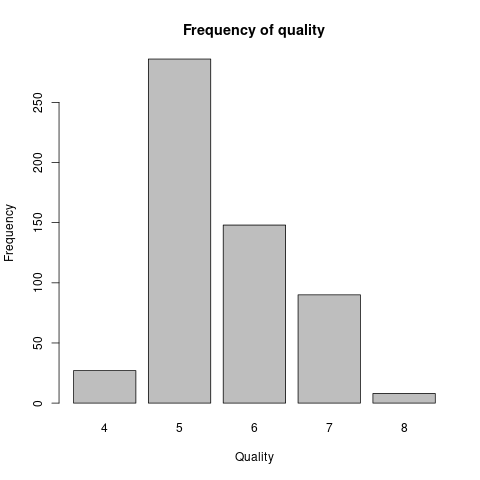
\includegraphics[width=0.8\textwidth]{../figures/quality-frequency.png}
                \label{fig:quality}
                \caption{酒品数据分布}
            \end{figure}

        \subsection{自变量描述}
            我们通过自变量与酒品的箱线图对其进行描述。下面展示部分具有代表性的数据。
            \clearpage
            \subsubsection{固定酸度(Fixed Acidity)}
                固定酸度关于酒品的箱线图如图所示。
                \begin{figure}[htbp]
                    \centering
                    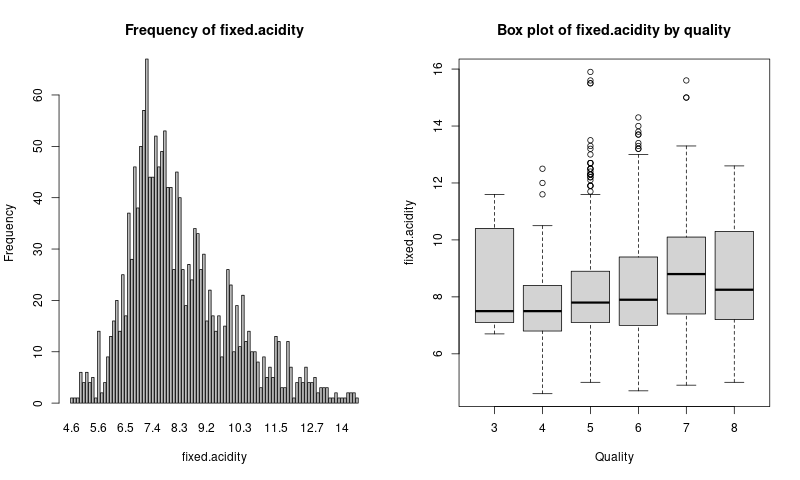
\includegraphics[width=0.8\textwidth]{../figures/fixed.acidity-plot.png}
                    \label{fig:fixed-acidity}
                    \caption{固定酸度箱线图}
                \end{figure}

            \subsubsection{挥发性酸度(Volatile Acidity)}
                挥发性酸度关于酒品的箱线图如图所示。
                \begin{figure}[htbp]
                    \centering
                    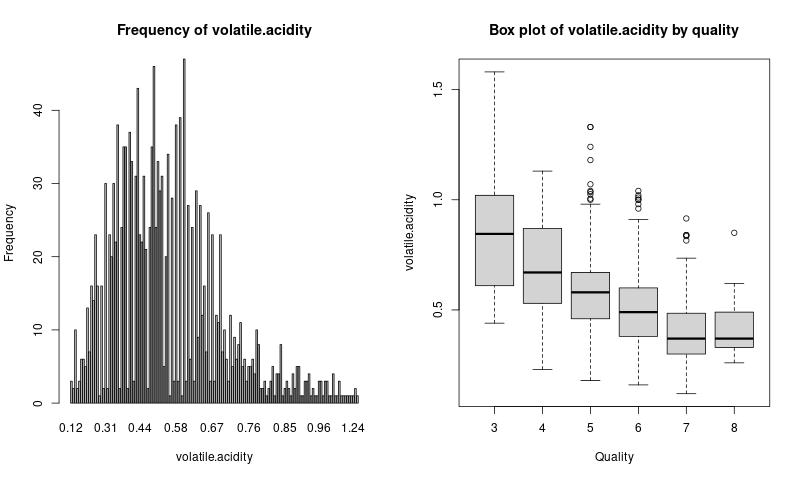
\includegraphics[width=0.8\textwidth]{../figures/volatile.acidity-plot.png}
                    \label{fig:volatile-acidity}
                    \caption{挥发性酸度分布箱线图}
                \end{figure}
            
            \subsubsection{游离二氧化硫(Free Sulfur Dioxide)}
                游离二氧化硫含量关于酒品的箱线图如图所示。
                \begin{figure}[htbp]
                    \centering
                    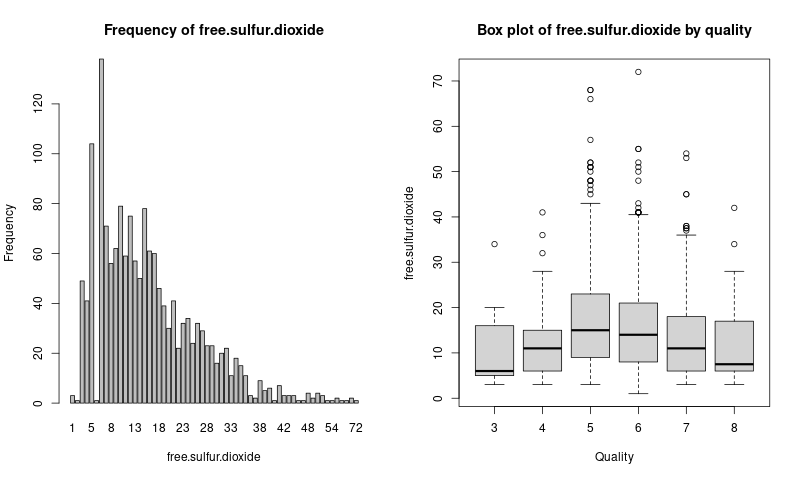
\includegraphics[width=0.8\textwidth]{../figures/free.sulfur.dioxide-plot.png}
                    \label{fig:free.sulfur.dioxide}
                    \caption{游离二氧化硫箱线图}
                \end{figure}   

            \subsubsection{醇度(Alcohol)}
                酒精含量关于酒品的箱线图如图所示。
                \begin{figure}[htbp]
                    \centering
                    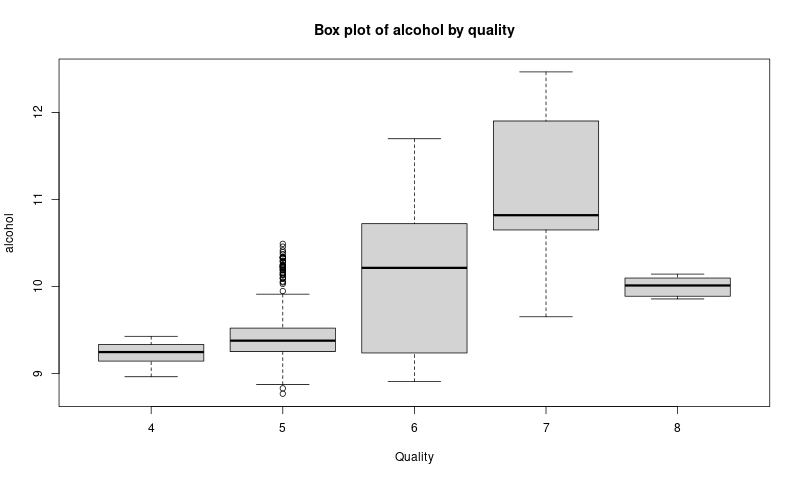
\includegraphics[width=0.8\textwidth]{../figures/alcohol-plot.png}
                    \label{fig:alcohol}
                    \caption{醇度箱线图}
                \end{figure} 
        
        \subsection{自变量相关性分析}
            我们对自变量相关性进行分析,结果如图所示。可以发现,与体现酒的酸碱性的自变量相关性相对较大,需要通过后续处理消除它们的复共线性。
            \begin{figure}[htbp]
                \centering
                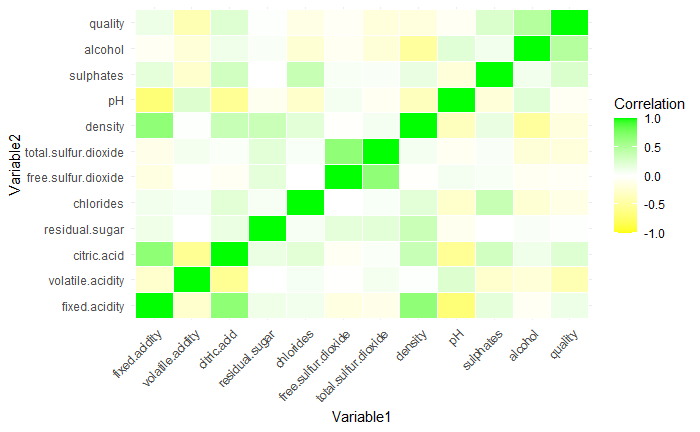
\includegraphics[width=0.8\textwidth]{../figures/covariance.png}
                \label{fig:covariance}
                \caption{自变量相关性热力图}
            \end{figure}
    \section{数据建模}
        我们首先使用线性模型全模型进行建模,通过红酒的化学成分特征,对酒品进行回归分析。为了减小异方差性,我们对响应变量Quality采用Box-cox变换。为了减少多重共线性,我们使用AIC、BIC准则以及主成分分析法对模型进行变量筛选。最后,为了弥补线性模型简单性导致的预测困难,我们使用多项式回归、广义线性模型和支持向量机进行预测。
        \clearpage
        \subsection{全模型}
            首先,我们对数据进行全模型最小二乘回归,得到结果如下:
            \begin{table}[htbp]
                \centering
                \begin{tabular}{rrrrl}
                    \hline
                    & Estimate & Std. Error & t value & Pr($>$$|$t$|$) \\ 
                    \hline
                    (Intercept) & 1.5577 & 0.8651 & 1.80 & 0.0723 . \\ 
                    fixed.acidity & 0.0771 & 0.0220 & 3.51 & 0.0005 *** \\ 
                    volatile.acidity & -1.0448 & 0.1477 & -7.07 & 0.0000 *** \\ 
                    citric.acid & 0.0886 & 0.1538 & 0.58 & 0.5648 \\ 
                    residual.sugar & 0.0100 & 0.0277 & 0.36 & 0.7174 \\ 
                    chlorides & -0.2167 & 0.1891 & -1.15 & 0.2523 \\ 
                    free.sulfur.dioxide & -0.0181 & 0.0044 & -4.10 & 0.0000 *** \\ 
                    total.sulfur.dioxide & -0.0008 & 0.0012 & -0.65 & 0.5157 \\ 
                    density & 0.1462 & 0.2437 & 0.60 & 0.5488 \\ 
                    pH & -0.2349 & 0.2072 & -1.13 & 0.2574 \\ 
                    sulphates & -0.0626 & 0.0550 & -1.14 & 0.2556 \\ 
                    alcohol & 0.4856 & 0.0376 & 12.91 & 0.0000 *** \\ 
                    \hline
                    \multicolumn{5}{c}{Residual standard error: 0.5762 on 547 degrees of freedom} \\
                    \multicolumn{5}{c}{Multiple R-squared:  0.5656,	Adjusted R-squared:  0.5569} \\
                    \multicolumn{5}{c}{F-statistic: 64.76 on 11 and 547 DF,  p-value: < 2.2e-16} \\
                    \hline
                \end{tabular}
                \label{tab:linear-model}
            \end{table}
            
            结果显示,在0.05的置信水平下,固定酸度、挥发性酸度、游离二氧化氮和醇度与酒品呈正相关。
            \clearpage
            然后我们对模型进行回归诊断,结果如下图:

            \begin{figure}[htbp]
                \centering
                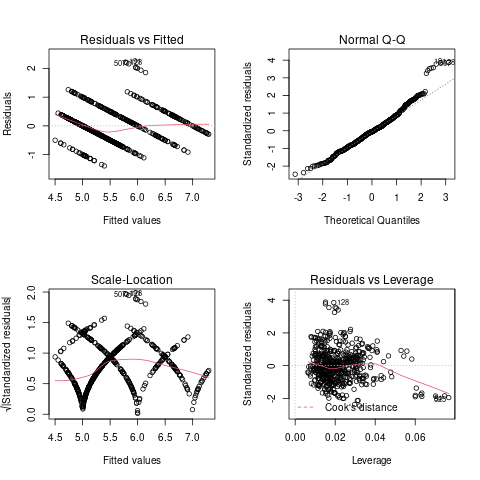
\includegraphics[width=0.8\textwidth]{../model-summary/linear-model-plot.png}
                \label{fig:linear-model}
                \caption{全模型诊断图}
            \end{figure}

            在左上角残差图中,有一部分离群点;
            在右上角Q-Q图中,有一部分数据发生了偏离;
            因此有必要对数据进一步处理。

            在进一步处理之前,我们先对模型进行一系列检验。
            \clearpage
            \subsubsection{异常值检验}
                利用Cook距离检验数据集中的异常值点,结果如下:
                \begin{figure}[htbp]
                    \centering
                    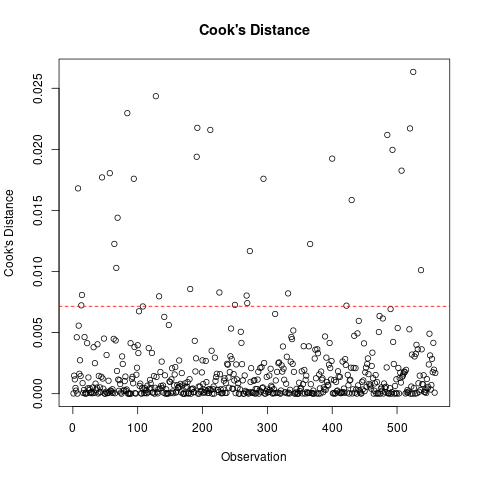
\includegraphics[width=0.8\textwidth]{../figures/cook.png}
                    \label{fig:cook}
                    \caption{Cook距离}
                \end{figure}
            
                可以看到,所有数据点的Cook距离都接近0。

            \subsubsection{异方差检验}
                利用ncvTest检验模型异方差性,结果如下:
                \begin{table}[htbp]
                    \centering
                    \caption{异方差检验}
                    \vspace{5pt}
                    \begin{tabular}{ccc}
                        \hline
                        Chisquare & Df & p \\
                        \hline
                        0.1033325 & 1 & 0.74787 \\
                        \hline
                    \end{tabular}
                \end{table}
                
                检验得到p值为0.74787,因此接受原假设,认为模型不具有异方差性。
               
            \subsubsection{自相关性检验}
                利用dwtest对误差自相关性进行检验,结果如下:
                \begin{table}[htbp]
                    \centering
                    \caption{自相关性检验}
                    \vspace{5pt}
                    \begin{tabular}{cc}
                        \hline
                        DW & p \\
                        \hline
                        2.0775 & 0.8176 \\
                        \hline
                    \end{tabular}
                \end{table}
                
                检验得到p值为0.8176,因此接受原假设,认为模型不具有自相关性。

            \subsubsection{多重共线性检验}
                利用VIF对自变量共线性进行检验,结果如下:
                \begin{table}[ht]
                    \centering
                    \caption{多重共线性}
                    \vspace{5pt}
                    \begin{tabular}{rr}
                        \hline
                        & VIF \\ 
                        \hline
                        fixed.acidity & 1.50 \\ 
                        volatile.acidity & 1.45 \\ 
                        citric.acid & 1.62 \\ 
                        residual.sugar & 1.75 \\ 
                        chlorides & 2.08 \\ 
                        free.sulfur.dioxide & 2.94 \\ 
                        total.sulfur.dioxide & 4.12 \\ 
                        density & 1.04 \\ 
                        pH & 2.08 \\ 
                        sulphates & 1.49 \\ 
                        alcohol & 1.62 \\ 
                        \hline
                    \end{tabular}
                \end{table}

                若VIF小于1,表示自变量不存在多重共线性的问题;若VIF在1到5之间,表示存在轻微的多重共线性问题;若VIF大于5,表示存在较强的多重共线性。可以看到,总二氧化硫可能与其他变量的相关性相对较强。
        \subsection{选模型}
            为了解决多重共线性的问题,我们通过AIC准则和BIC准则选取变量。
            \subsubsection{AIC准则}
                使用AIC准则选择变量,结果如下:

                \begin{table}[ht]
                    \centering
                    \begin{tabular}{rrrrl}
                        \hline
                        & Estimate & Std. Error & t value & Pr($>$$|$t$|$) \\ 
                        \hline
                        (Intercept) & 0.6495 & 0.3696 & 1.76 & 0.0794 . \\ 
                        fixed.acidity & 0.0952 & 0.0190 & 5.01 & 7.46e-07 *** \\ 
                        volatile.acidity & -1.0721 & 0.1330 & -8.06 & 4.78e-15 *** \\ 
                        free.sulfur.dioxide & -0.0201 & 0.0026 & -7.66 & 8.48e-14 *** \\ 
                        alcohol & 0.4991 & 0.0329 & 15.16 & < 2e-16 *** \\ 
                        \hline
                        \multicolumn{5}{c}{Residual standard error: 0.5743 on 554 degrees of freedom} \\
                        \multicolumn{5}{c}{Multiple R-squared:  0.563,	Adjusted R-squared:  0.5598 } \\
                        \multicolumn{5}{c}{F-statistic: 178.4 on 4 and 554 DF,  p-value: < 2.2e-16} \\
                        \hline
                    \end{tabular}
                \end{table}

            \subsubsection{BIC准则}
                使用BIC准则选择变量,结果如下:

                \begin{table}[ht]
                    \centering
                    \begin{tabular}{rrrrl}
                        \hline
                        & Estimate & Std. Error & t value & Pr($>$$|$t$|$) \\ 
                        \hline
                        (Intercept) & 0.6495 & 0.3696 & 1.76 & 0.0794 . \\ 
                        fixed.acidity & 0.0952 & 0.0190 & 5.01 & 7.46e-07 *** \\ 
                        volatile.acidity & -1.0721 & 0.1330 & -8.06 & 4.78e-15 *** \\ 
                        free.sulfur.dioxide & -0.0201 & 0.0026 & -7.66 & 8.48e-14 *** \\ 
                        alcohol & 0.4991 & 0.0329 & 15.16 & < 2e-16 *** \\ 
                        \hline
                        \multicolumn{5}{c}{Residual standard error: 0.5743 on 554 degrees of freedom} \\
                        \multicolumn{5}{c}{Multiple R-squared:  0.563,	Adjusted R-squared:  0.5598 } \\
                        \multicolumn{5}{c}{F-statistic: 178.4 on 4 and 554 DF,  p-value: < 2.2e-16} \\
                        \hline
                    \end{tabular}
                \end{table}

                使用AIC准则和BIC准则筛选出来的变量相同。
        
        \clearpage
        \subsection{Box-cox变换}
            为了改善数据的非正态性与异方差性,我们对Quality进行Box-cox变换。
            \begin{figure}[htbp]
                \centering
                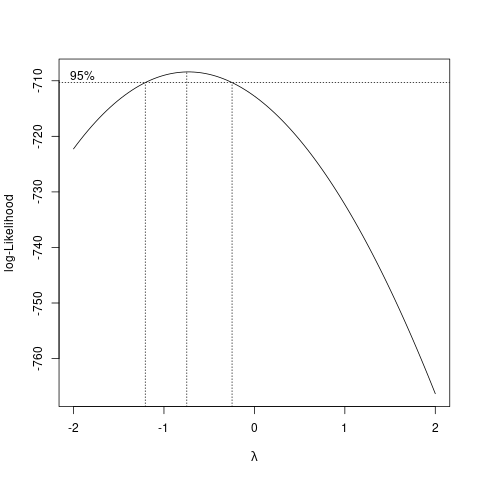
\includegraphics[width=0.8\textwidth]{../figures/boxcox.png}
                \label{fig:boxcox}
                \caption{box-cox变换}
            \end{figure}

            当 $\lambda = -0.74747$ 时,对数似然函数达到最大值。

        \subsection{主成份分析}
            我们可以使用主成份分析法进一步降低模型多重共线性。
            \begin{table}[ht]
                \centering
                \begin{tabular}{rrrrrrr}
                    \hline
                    & PC1 & PC2 & PC3 & PC4 & PC5 & PC6 \\ 
                    \hline
                    Standard deviation & 1.7721 & 1.5014 & 1.1901 & 1.0942 & 0.9574 & 0.9279 \\ 
                    Proportion of Variance & 0.2617 & 0.1878 & 0.1180 & 0.0998 & 0.0764 & 0.0717  \\ 
                    Cumulative Proportion & 0.2617 & 0.4496 & 0.5676 & 0.6674 & 0.7438 & 0.8155 \\ 
                    \hline
                \end{tabular}
            \end{table}
            
            前六个主成分贡献了近 $80\%$ 的方差。

        \subsection{多项式回归}
            线性模型的$R^2$在0.56左右,我们尝试对特征做非线性变换进行拟合,
            考虑增加二次项以及交叉项,结果如表 \ref{tab:poly} 所示。
            \begin{table}[ht]
                \centering
                \begin{tabular}{rrrrl}
                    \hline
                    & Estimate & Std. Error & t value & Pr($>$$|$t$|$) \\ 
                    \hline
                    (Intercept) & 5.1919 & 8.0083 & 0.65 & 0.5171 \\ 
                    fixed.acidity & -0.6923 & 0.2256 & -3.07 & 0.0023 ** \\ 
                    volatile.acidity & -2.3077 & 0.5931 & -3.89 & 0.0001 *** \\ 
                    citric.acid & 2.9554 & 0.4191 & 7.05 & 0.0000 *** \\ 
                    residual.sugar & -0.6555 & 0.1427 & -4.59 & 0.0000 *** \\ 
                    chlorides & 0.6627 & 0.3489 & 1.90 & 0.0581 . \\ 
                    free.sulfur.dioxide & 0.0267 & 0.0156 & 1.71 & 0.0878 . \\ 
                    total.sulfur.dioxide & -0.0181 & 0.0045 & -4.02 & 0.0001 *** \\ 
                    density & 0.7788 & 3.2565 & 0.24 & 0.8111 \\ 
                    pH & -8.2459 & 4.2524 & -1.94 & 0.0530 . \\ 
                    sulphates & 0.4413 & 0.1646 & 2.68 & 0.0076 ** \\ 
                    alcohol & 2.9686 & 0.7301 & 4.07 & 0.0001 *** \\ 
                    fixed.acidity.2 & 0.0391 & 0.0118 & 3.32 & 0.0010 *** \\ 
                    volatile.acidity.2 & 1.4698 & 0.5560 & 2.64 & 0.0084 ** \\ 
                    citric.acid.2 & -2.8046 & 0.4432 & -6.33 & 0.0000 *** \\ 
                    residual.sugar.2 & 0.0839 & 0.0186 & 4.51 & 0.0000 *** \\ 
                    chlorides.2 & -1.1154 & 0.6064 & -1.84 & 0.0664 .\\ 
                    free.sulfur.dioxide.2 & -0.0008 & 0.0004 & -2.14 & 0.0329 * \\ 
                    total.sulfur.dioxide.2 & 0.0001 & 0.0000 & 3.49 & 0.0005 *** \\ 
                    density.2 & -0.2608 & 1.6167 & -0.16 & 0.8719 \\ 
                    pH.2 & 1.1943 & 0.6806 & 1.75 & 0.0799 . \\ 
                    sulphates.2 & -0.1783 & 0.0632 & -2.82 & 0.0050 ** \\ 
                    alcohol.2 & -0.1132 & 0.0347 & -3.27 & 0.0012 ** \\ 
                    \hline
                    \multicolumn{5}{c}{Residual standard error: 0.5211 on 536 degrees of freedom} \\
                    \multicolumn{5}{c}{Multiple R-squared:  0.6518,	Adjusted R-squared:  0.6375 } \\
                    \multicolumn{5}{c}{F-statistic:  45.6 on 22 and 536 DF,  p-value: < 2.2e-16} \\
                    \hline
                \end{tabular}
                \caption{多项式回归}
                \label{tab:poly}
            \end{table}

            增加二次项后,模型$R^2$增加约0.1,残差标准差从0.5762降到0.5211。

        
        \subsection{广义线性模型}
            我们基于增加了二次项的数据进行广义线性模型回归。假设$ y \sim N(\mu, \sigma^2)$,使用广义线性模型对 $y$ 进行预测,结果如表 \ref{tab:glm} 所示。在测试数据集上,该模型达到了$69.52\%$的精度。
            \begin{table}[ht]
                \centering
                \begin{tabular}{rrrrr}
                    \hline
                    & Estimate & Std. Error & t value & Pr($>$$|$t$|$) \\ 
                    \hline
                    (Intercept) & 5.1919 & 8.0083 & 0.65 & 0.5171 \\ 
                    fixed.acidity & -0.6923 & 0.2256 & -3.07 & 0.0023 \\ 
                    volatile.acidity & -2.3077 & 0.5931 & -3.89 & 0.0001 \\ 
                    citric.acid & 2.9554 & 0.4191 & 7.05 & 0.0000 \\ 
                    residual.sugar & -0.6555 & 0.1427 & -4.59 & 0.0000 \\ 
                    chlorides & 0.6627 & 0.3489 & 1.90 & 0.0581 \\ 
                    free.sulfur.dioxide & 0.0267 & 0.0156 & 1.71 & 0.0878 \\ 
                    total.sulfur.dioxide & -0.0181 & 0.0045 & -4.02 & 0.0001 \\ 
                    density & 0.7788 & 3.2565 & 0.24 & 0.8111 \\ 
                    pH & -8.2459 & 4.2524 & -1.94 & 0.0530 \\ 
                    sulphates & 0.4413 & 0.1646 & 2.68 & 0.0076 \\ 
                    alcohol & 2.9686 & 0.7301 & 4.07 & 0.0001 \\ 
                    fixed.acidity.2 & 0.0391 & 0.0118 & 3.32 & 0.0010 \\ 
                    volatile.acidity.2 & 1.4698 & 0.5560 & 2.64 & 0.0084 \\ 
                    citric.acid.2 & -2.8046 & 0.4432 & -6.33 & 0.0000 \\ 
                    residual.sugar.2 & 0.0839 & 0.0186 & 4.51 & 0.0000 \\ 
                    chlorides.2 & -1.1154 & 0.6064 & -1.84 & 0.0664 \\ 
                    free.sulfur.dioxide.2 & -0.0008 & 0.0004 & -2.14 & 0.0329 \\ 
                    total.sulfur.dioxide.2 & 0.0001 & 0.0000 & 3.49 & 0.0005 \\ 
                    density.2 & -0.2608 & 1.6167 & -0.16 & 0.8719 \\ 
                    pH.2 & 1.1943 & 0.6806 & 1.75 & 0.0799 \\ 
                    sulphates.2 & -0.1783 & 0.0632 & -2.82 & 0.0050 \\ 
                    alcohol.2 & -0.1132 & 0.0347 & -3.27 & 0.0012 \\ 
                    \hline
                    \multicolumn{5}{c}{Null deviance: 418.05  on 558  degrees of freedom} \\
                    \multicolumn{5}{c}{Residual deviance: 145.57  on 536  degrees of freedom} \\
                    \multicolumn{5}{c}{AIC: 882.26} \\
                    \multicolumn{5}{c}{Number of Fisher Scoring iterations: 2} \\
                    \hline
                \end{tabular}
                \caption{广义线性模型}
                \label{tab:glm}
            \end{table}

        \subsection{支持向量机}
            使用高斯核函数
            \[ K(x, y) = \exp\left(-\frac{\|x - y\|^2}{2\sigma^2}\right) \]
            并设置参数 $\gamma$ 和 $cost$ 的参数搜索空间,搜索结果如图 \ref{fig:svm} 所示,得到$cost = 10, \gamma = 0.1$ 时模型效果最好,达到了 $82.89\%$ 的精度。

            \begin{figure}[htbp]
                \centering
                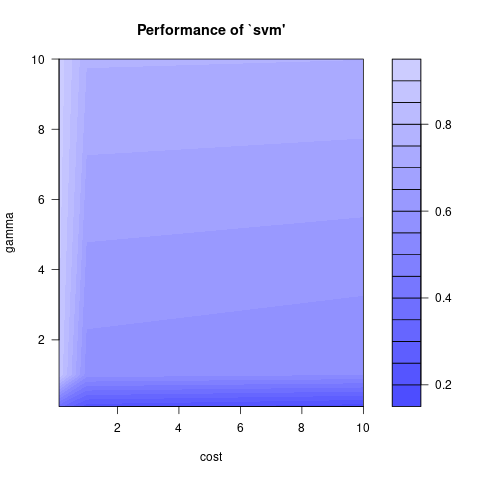
\includegraphics[width=0.5\textwidth]{../model-summary/svm.png}
                \label{fig:svm}
                \caption{SVM参数空间}
            \end{figure}
        \clearpage
    \section{结论及建议}
        基于若干种不同的统计模型,我们对酒品的影响因素做了全面的分析。通过分析这些关键特征与酒的品质之间的关系,我们可以更好地理解这些特征如何影响酒的品质和消费者的感知。这种深入的分析有助于酿酒业者优化酒的配方和生产流程,以满足不同口味偏好的消费者需求。此外,对于消费者而言,了解这些特征的影响可以帮助他们更明智地选择适合自己口味的酒类产品。
        总体而言,酒的酸度、醇度以及$SO_2$含量对于酒的品质较为重要。
    
    \section{缺陷与改进}
        尽管我们的回归分析为我们提供了一些对因变量的理解,但我们也要意识到分析中存在一些缺陷和局限性。

        在真实的数据中,酒的品质的影响因素是多种多样的,我们的模型可能过于简化了问题,未能充分考虑所有潜在的影响因素。
        实际上,除了酒的物理、化学性质以外,还有很多重要的影响因素没有被考虑到,这需要我们进一步收集相关数据,增强模型的解释性。

        此外,由品酒师的主观感受对酒的品质进行量化可能导致结果不够客观。如果可以找到一个更客观的评价标准,那么数据的准确性就能够增加。
    \newpage
    \bibliographystyle{plain}
    \bibliography{ref} 

\end{document}